% Paytm Hisaab -- Round 1 idea proposal
% Paytm Build for India AI Hackathon, Bengaluru Edition. Track 3: Autonomous AI Teammates.
%
% Covers the seven required sections: Title, Problem Statement, Proposed Solution,
% Technology Stack, USP, Impact & Benefits, Business Model.
% One message per slide, short phrases, large type: it should read at a glance.
%
% Compile with XeLaTeX (needed for the rupee sign), twice so the page total resolves:
%
%   xelatex hisaab-proposal.tex && xelatex hisaab-proposal.tex
%
% Fonts: Segoe UI (ships with Windows). Elsewhere it falls back to the default sans.
\documentclass[aspectratio=169,10pt]{beamer}

\usepackage{fontspec}
\usepackage{amssymb}
\usepackage{tikz}
\usepackage{array}
\newcolumntype{L}[1]{>{\raggedright\arraybackslash}p{#1}}
\usetikzlibrary{calc,positioning,arrows.meta}

% ---------- team (fill in; left empty, nothing is printed) ----------
\def\teamname{}
\def\teammembers{}

% ---------- fonts ----------
\IfFontExistsTF{Segoe UI}{\setsansfont{Segoe UI}}{}
\renewcommand{\familydefault}{\sfdefault}

\hyphenpenalty=10000
\exhyphenpenalty=10000
\emergencystretch=3em
\hbadness=10000

% ---------- palette ----------
\definecolor{navy}{HTML}{002970}
\definecolor{ptmcyan}{HTML}{00BAF2}
\definecolor{ink}{HTML}{0F172A}
\definecolor{muted}{HTML}{64748B}
\definecolor{good}{HTML}{15803D}
\definecolor{bad}{HTML}{DC2626}
\definecolor{amber}{HTML}{B45309}
\definecolor{tint}{HTML}{EAF4FD}
\definecolor{hairline}{HTML}{DBE7F3}

% ---------- theme ----------
\usetheme{default}
\usecolortheme{default}
\setbeamertemplate{navigation symbols}{}
\setbeamersize{text margin left=0.85cm,text margin right=0.85cm}
\setbeamercolor{normal text}{fg=ink,bg=white}
\setbeamercolor{frametitle}{fg=navy}
\setbeamercolor{structure}{fg=navy}
\setbeamerfont{frametitle}{size=\Large,series=\bfseries}

% the required-section label printed above every frame title
\def\secttag{}
\newcommand{\sect}[1]{\def\secttag{#1}}
\setbeamertemplate{frametitle}{%
  \vspace{0.25cm}%
  {\fontsize{7}{8}\selectfont\bfseries\color{ptmcyan}\secttag}\par\vspace{0.1em}%
  \usebeamerfont{frametitle}\usebeamercolor[fg]{frametitle}\insertframetitle\par\vspace{0.15em}%
  {\color{ptmcyan}\rule{1.2cm}{2pt}}\par\vspace{-0.2cm}%
}
\setbeamertemplate{footline}{%
  \hbox{\begin{beamercolorbox}[wd=\paperwidth,ht=1.9ex,dp=1.1ex,leftskip=0.85cm,rightskip=0.85cm]{}%
  {\scriptsize\color{muted}\hfill\insertframenumber\,/\,\inserttotalframenumber}%
  \end{beamercolorbox}}%
}

% ---------- helpers ----------
\newcommand{\hi}[1]{\leavevmode{\color{navy}\bfseries #1}}
\newcommand{\qm}[1]{``#1''}
% bullet and check with a hanging indent
\newcommand{\bpt}[1]{{\hangindent=0.9em\hangafter=1\noindent\makebox[0.9em][l]{\color{ptmcyan}\textbullet}#1\par}\vspace{0.3em}}
\newcommand{\chk}[1]{{\hangindent=1.4em\hangafter=1\noindent\makebox[1.4em][l]{\color{good}\large$\checkmark$}#1\par}\vspace{0.9em}}
% \boxcard{fill}{draw}{width}{height or empty}{body}; top-aligned so cards in a row line up
\newcommand{\boxcard}[5]{%
  \begin{tikzpicture}[baseline=(current bounding box.north)]%
  \node[rounded corners=5pt,fill=#1,draw=#2,line width=1pt,inner sep=8pt,font=\small]{%
    \if\relax\detokenize{#4}\relax\begin{minipage}{#3}\else\begin{minipage}[t][#4][t]{#3}\fi
    \raggedright #5\end{minipage}};%
  \end{tikzpicture}}
\newcommand{\card}[3][]{\boxcard{tint}{none}{#2}{#1}{#3}}
\newcommand{\ocard}[4][]{\boxcard{white}{#2}{#3}{#1}{#4}}
\newcommand{\ncard}[3][]{\boxcard{navy}{none}{#2}{#1}{\color{white}#3}}
% big number:  \stat{colour}{number}{label}
\newcommand{\stat}[3]{\ocard{#1}{3.95cm}{\centering{\fontsize{28}{30}\selectfont\bfseries\color{#1}#2\par}\vspace{0.25em}{\color{muted}#3\par}}}
% heading + short line:  \tile{width}{height}{heading}{body}
\newcommand{\tile}[4]{\card[#2]{#1}{{\normalsize\bfseries\color{navy}#3\par}\vspace{0.3em}#4}}
% a workflow lane:  \lane{colour}{title}{step 1}{step 2}{step 3}
\newcommand{\step}[3]{{\hangindent=1.1em\hangafter=1\noindent\makebox[1.1em][l]{\color{#1}\bfseries #2}#3\par}\vspace{0.4em}}
\newcommand{\lane}[5]{\ocard[2.35cm]{#1}{3.95cm}{{\large\bfseries\color{#1}#2\par}\vspace{0.6em}\step{#1}{1}{#3}\step{#1}{2}{#4}\step{#1}{3}{#5}}}

\tikzset{
  hbx/.style={rounded corners=4pt,fill=tint,inner sep=6pt,align=left,font=\footnotesize,text width=#1},
  flow/.style={-{Stealth[length=2.2mm]},ptmcyan,line width=1.3pt},
}

\begin{document}

% ============================================================ 1. TITLE
{\setbeamertemplate{footline}{}
\begin{frame}[plain]
\vspace{0.5cm}
\begin{center}
{\scriptsize\bfseries\color{ptmcyan}IDEA PROPOSAL \;$\cdot$\; ROUND 1}\\[1em]
{\fontsize{40}{44}\selectfont\bfseries\color{navy}Paytm\;\color{ink}Hisaab}\\[0.5em]
{\Large\color{muted}Every rupee, on your side.}\\[1em]
{\color{ptmcyan}\rule{2.8cm}{2.5pt}}\\[1em]
{\large\color{ink}An AI teammate that explains a merchant's money}\\[0.2em]
{\large\color{ink}when a freeze or a tax notice hits.}\\[1.4em]
{\small\color{muted}Track 3: Autonomous AI Teammates \;$\cdot$\; Paytm Build for India AI Hackathon, Bengaluru}\\[0.45em]
{\scriptsize\color{muted}Built on n8n \;$\cdot$\; Sarvam AI \;$\cdot$\; Cognee}
\ifx\teamname\empty\else\\[0.9em]{\small\bfseries\color{navy}Team \teamname}\fi
\ifx\teammembers\empty\else\\[0.2em]{\scriptsize\color{muted}\teammembers}\fi
\end{center}
\end{frame}}

% ============================================================ 2. PROBLEM: THE CONTEXT
\sect{PROBLEM STATEMENT}
\begin{frame}{Small merchants can't explain their own UPI money}
\vspace{0.35cm}
{\centering
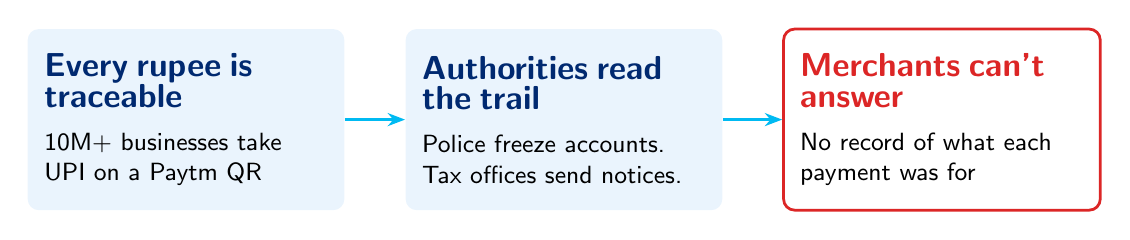
\begin{tikzpicture}
\tikzset{ctx/.style={hbx=3.6cm,minimum height=2.3cm,font=\small}}
\node[ctx] (a) at (0,0)
  {{\large\bfseries\color{navy}Every rupee is traceable}\\[0.5em]10M+ businesses take UPI on a Paytm QR};
\node[ctx] (b) at (4.8,0)
  {{\large\bfseries\color{navy}Authorities read the trail}\\[0.5em]Police freeze accounts. Tax offices send notices.};
\node[ctx,fill=white,draw=bad,line width=1pt] (c) at (9.6,0)
  {{\large\bfseries\color{bad}Merchants can't answer}\\[0.5em]No record of what each payment was for};
\draw[flow] (a) -- (b); \draw[flow] (b) -- (c);
\end{tikzpicture}\par}
\vspace{0.7cm}
{\centering\ncard{13.2cm}{\centering\normalsize The result: \textbf{frozen accounts, wrong tax bills, and shops going back to cash.}}\par}
\end{frame}

% ============================================================ 3. PROBLEM: A TYPICAL FREEZE
\sect{PROBLEM STATEMENT \;$\cdot$\; A TYPICAL CASE}
\begin{frame}{One payment can freeze a whole shop}
\vspace{0.2cm}
\noindent\stat{bad}{₹4,200}{the disputed payment}\hfill
\stat{navy}{339}{payments that week}\hfill
\stat{bad}{100\%}{of the account frozen}
\par\vspace{0.5cm}
{\centering\small They sold onions to a customer three hops from a fraud. They aren't even named in the FIR.\par}
\vspace{0.45cm}
\noindent\card{3.95cm}{{\bfseries\color{navy}The bank}\par has no bill}\hfill
\card{3.95cm}{{\bfseries\color{navy}The police officer}\par is in another state}\hfill
\card{3.95cm}{{\bfseries\color{navy}The merchant}\par can't find the payment}
\par\vspace{0.4cm}
{\centering\normalsize\hi{Nobody can say which payment it was, or what it paid for.}\par}
\end{frame}

% ============================================================ 3. PROBLEM: TWO AUTHORITIES
\sect{PROBLEM STATEMENT}
\begin{frame}{Two authorities now demand an answer}
\vspace{0.2cm}
\noindent\card[3.35cm]{6.4cm}{{\large\bfseries\color{bad}Cyber-crime freezes\par}
  {\footnotesize\color{muted}MHA and I4C SOP, January 2026\par}\vspace{0.5em}
  \bpt{Freeze only the disputed amount}
  \bpt{Tell mules apart from genuine sellers}
  \bpt{Release small sums once the trail is verified}
  \vspace{0.1em}{\footnotesize\color{muted}Andhra Pradesh and Rajasthan High Courts ruled the same way in 2026.\par}}\hfill
\card[3.35cm]{6.4cm}{{\large\bfseries\color{amber}GST notices\par}
  {\footnotesize\color{muted}Haveri, Karnataka, 2025\par}\vspace{0.4em}
  {\centering{\fontsize{30}{32}\selectfont\bfseries\color{bad}₹29 lakh\par}}\vspace{0.4em}
  demanded from a vegetable seller whose sales were tax-exempt\par\vspace{0.4em}
  {\footnotesize\color{muted}Similar notices are still going out in 2026.\par}}
\par\vspace{0.45cm}
{\centering\ncard{13.2cm}{\centering\normalsize Both ask one question: \textbf{what was each rupee, actually?}}\par}
\end{frame}

% ============================================================ 4. SOLUTION: ONE LEDGER
\sect{PROPOSED SOLUTION}
\begin{frame}{One ledger, two answers}
\vspace{0.3cm}
{\centering
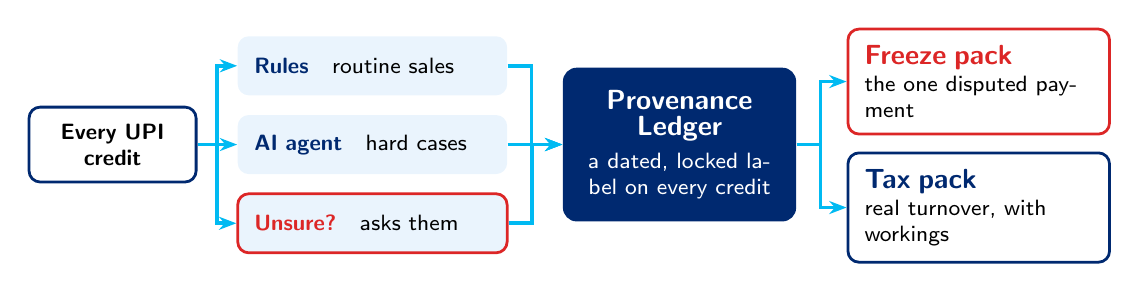
\begin{tikzpicture}
\node[hbx=1.7cm,fill=white,draw=navy,line width=1pt,align=center,font=\footnotesize\bfseries] (src) at (0,0) {Every UPI credit};
\node[hbx=3.0cm,minimum height=0.75cm] (rules) at (3.3,1.0)  {{\bfseries\color{navy}Rules}\quad routine sales};
\node[hbx=3.0cm,minimum height=0.75cm] (ai)    at (3.3,0)    {{\bfseries\color{navy}AI agent}\quad hard cases};
\node[hbx=3.0cm,minimum height=0.75cm,draw=bad,line width=1pt] (ask) at (3.3,-1.0) {{\bfseries\color{bad}Unsure?}\quad asks them};
\node[rounded corners=5pt,fill=navy,text=white,inner sep=8pt,align=center,text width=2.4cm,font=\footnotesize] (led) at (7.2,0)
  {{\normalsize\bfseries Provenance Ledger}\\[0.3em]a dated, locked label on every credit};
\node[hbx=2.9cm,fill=white,draw=bad,line width=1pt] (o1) at (11.0,0.8)
  {{\normalsize\bfseries\color{bad}Freeze pack}\\the one disputed payment};
\node[hbx=2.9cm,fill=white,draw=navy,line width=1pt] (o2) at (11.0,-0.8)
  {{\normalsize\bfseries\color{navy}Tax pack}\\real turnover, with workings};
\foreach \n in {rules,ai,ask} {
  \draw[flow] (src.east) -- ++(0.25,0) |- (\n.west);
  \draw[flow] (\n.east) -- ++(0.3,0) |- (led.west);
}
\draw[flow] (led.east) -- ++(0.3,0) |- (o1.west);
\draw[flow] (led.east) -- ++(0.3,0) |- (o2.west);
\end{tikzpicture}\par}
\vspace{0.75cm}
{\centering\normalsize It never guesses: \hi{at most 3 questions a day}, one tap each, in their own language.\par}
\end{frame}

% ============================================================ 5. SOLUTION: END TO END
\sect{PROPOSED SOLUTION}
\begin{frame}{The teammate works each case end to end}
\vspace{0.2cm}
\noindent\lane{navy}{Every night}{Labels new payments}{Asks up to 3 questions}{Warns before the GST limit}\hfill
\lane{bad}{Account frozen}{Finds the one payment}{Builds the evidence}{Drafts the grievance}\hfill
\lane{amber}{Tax notice}{Reads the notice}{Rebuilds real turnover}{Explains it to their CA}
\par\vspace{0.5cm}
\noindent\card{13.6cm}{{\bfseries\color{bad}Hands to a human} when evidence is weak, the amount is large, or they dispute a label.\par\vspace{0.25em}
{\bfseries\color{navy}Nothing is sent without a Paytm officer's approval.}}
\end{frame}

% ============================================================ 6. SOLUTION: TRACK 3 FIT
\sect{PROPOSED SOLUTION}
\begin{frame}{A teammate, not a chatbot}
\vspace{0.05cm}
{\normalsize\bfseries\color{ink}It understands, decides, acts, and knows when to hand over\par}
\vspace{0.35cm}
\noindent\tile{3.95cm}{1.45cm}{Understands context}{Remembers each shop}\hfill
\tile{3.95cm}{1.45cm}{Makes decisions}{Picks 1 payment out of 339}\hfill
\tile{3.95cm}{1.45cm}{Takes actions}{Builds packs, drafts grievances}
\par\vspace{0.3cm}
\noindent\tile{3.95cm}{1.45cm}{Works with humans}{They confirm, an officer approves}\hfill
\tile{3.95cm}{1.45cm}{Escalates wisely}{Only weak or large cases}\hfill
\tile{3.95cm}{1.45cm}{Measurable outcomes}{Days to release, merchants kept}
\end{frame}

% ============================================================ 7. SOLUTION: TRUST
\sect{PROPOSED SOLUTION}
\begin{frame}{A record nobody can fake later}
\vspace{0.25cm}
\begin{columns}[T]
\begin{column}{0.43\textwidth}
\vspace{0.35cm}
{\normalsize
\chk{Append-only and hash-chained}
\chk{A daily fingerprint anchored outside Paytm}
\chk{Their answers never overwrite the AI's label}
\chk{No one can backdate a history}}
\end{column}
\begin{column}{0.53\textwidth}
{\normalsize\bfseries\color{navy}Every line of the pack is graded\par}\vspace{0.5em}
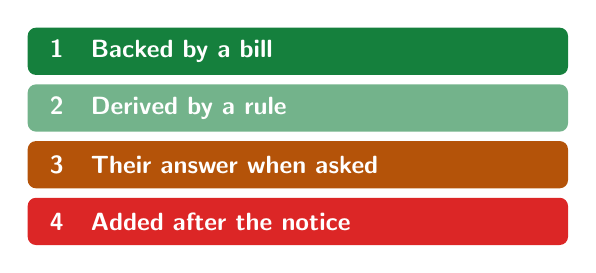
\begin{tikzpicture}
\foreach \c/\t [count=\k] in {good/Backed by a bill, good!60/Derived by a rule, amber/Their answer when asked, bad/Added after the notice} {
  \node[fill=\c,text=white,rounded corners=3pt,text width=6.3cm,minimum height=0.6cm,align=left,anchor=north west,inner xsep=8pt,font=\small\bfseries]
    at (0,-0.72*\k) {\k\quad\t};
}
\end{tikzpicture}\par\vspace{0.4em}
{\small\color{muted}Real shops: mostly 1 and 2. Fakes: mostly 3 and 4.\par}
\end{column}
\end{columns}
\vspace{0.55cm}
{\centering\large\hi{We sort. We don't advocate.}\par}
\end{frame}

% ============================================================ 8. TECH: ARCHITECTURE
\sect{TECHNOLOGY STACK}
\begin{frame}{Architecture}
\vspace{0.25cm}
{\centering
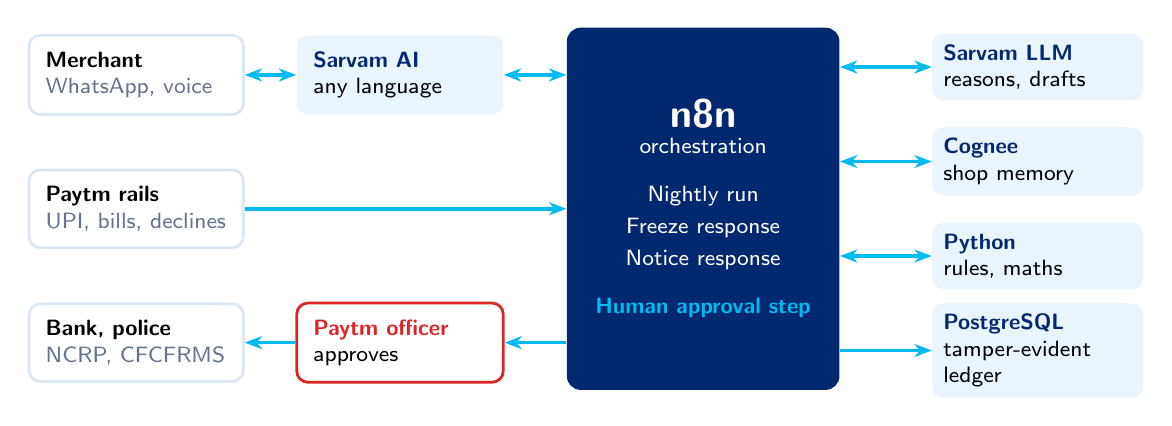
\begin{tikzpicture}
\tikzset{
  actor/.style={hbx=2.3cm,fill=white,draw=hairline,line width=1pt},
  svc/.style={hbx=2.4cm,inner sep=4pt},
  flow2/.style={{Stealth[length=2.2mm]}-{Stealth[length=2.2mm]},ptmcyan,line width=1.3pt},
}
\node[actor] (mer)   at (0,1.7)  {{\bfseries Merchant}\\{\color{muted}WhatsApp, voice}};
\node[actor] (rails) at (0,0)    {{\bfseries Paytm rails}\\{\color{muted}UPI, bills, declines}};
\node[actor] (auth)  at (0,-1.7) {{\bfseries Bank, police}\\{\color{muted}NCRP, CFCFRMS}};
\node[hbx=2.2cm] (sar) at (3.35,1.7) {{\bfseries\color{navy}Sarvam AI}\\any language};
\node[hbx=2.2cm,fill=white,draw=bad,line width=1pt] (off) at (3.35,-1.7) {{\bfseries\color{bad}Paytm officer}\\approves};
\node[rounded corners=5pt,fill=navy,text=white,inner sep=8pt,align=center,text width=2.9cm,minimum height=4.6cm,font=\footnotesize] (n8n) at (7.2,0)
  {{\Large\bfseries n8n}\\orchestration\\[0.9em]
   Nightly run\\[0.25em]Freeze response\\[0.25em]Notice response\\[0.9em]
   {\color{ptmcyan}\bfseries Human approval step}};
\node[svc] (llm) at (11.45,1.8)  {{\bfseries\color{navy}Sarvam LLM}\\reasons, drafts};
\node[svc] (cog) at (11.45,0.6)  {{\bfseries\color{navy}Cognee}\\shop memory};
\node[svc] (py)  at (11.45,-0.6) {{\bfseries\color{navy}Python}\\rules, maths};
\node[svc] (db)  at (11.45,-1.8) {{\bfseries\color{navy}PostgreSQL}\\tamper-evident ledger};
\draw[flow2] (mer.east) -- (sar.west);
\draw[flow2] (sar.east) -- (sar.east -| n8n.west);
\draw[flow]  (rails.east) -- (rails.east -| n8n.west);
\draw[flow]  (n8n.west |- off.east) -- (off.east);
\draw[flow]  (off.west) -- (auth.east);
\draw[flow2] (n8n.east |- llm.west) -- (llm.west);
\draw[flow2] (n8n.east |- cog.west) -- (cog.west);
\draw[flow2] (n8n.east |- py.west) -- (py.west);
\draw[flow]  (n8n.east |- db.west) -- (db.west);
\end{tikzpicture}\par}
\vspace{0.5cm}
{\centering\small Every step is an n8n node you can open and inspect. \hi{Only a person sends anything out.}\par}
\end{frame}

% ============================================================ 9. TECH STACK
\sect{TECHNOLOGY STACK}
\begin{frame}{Built on n8n, Sarvam AI and Cognee}
\vspace{0.2cm}
\noindent\tile{3.95cm}{1.1cm}{\large n8n}{{\color{muted}runs every workflow}}\hfill
\tile{3.95cm}{1.1cm}{\large Sarvam AI}{{\color{muted}LLM in their language}}\hfill
\tile{3.95cm}{1.1cm}{\large Cognee}{{\color{muted}remembers each shop}}
\par\vspace{0.3cm}
\noindent\tile{3.95cm}{1.1cm}{\large Python + FastAPI}{{\color{muted}does all the maths}}\hfill
\tile{3.95cm}{1.1cm}{\large PostgreSQL}{{\color{muted}the tamper-evident ledger}}\hfill
\tile{3.95cm}{1.1cm}{\large WhatsApp}{{\color{muted}where they already are}}
\par\vspace{0.55cm}
{\centering

\begin{tikzpicture}[font=\small]
\node[hbx=2.6cm,align=center] (a) at (0,0)    {\bfseries AI proposes};
\node[hbx=2.6cm,align=center] (b) at (3.6,0)  {\bfseries Python calculates};
\node[hbx=2.6cm,align=center] (c) at (7.2,0)  {\bfseries Ledger records};
\node[hbx=2.6cm,align=center,fill=navy,text=white] (d) at (10.8,0) {\bfseries A person approves};
\draw[flow] (a) -- (b); \draw[flow] (b) -- (c); \draw[flow] (c) -- (d);
\end{tikzpicture}\par}
\end{frame}

% ============================================================ 9. USP
\sect{USP}
\begin{frame}{Why only Paytm can do this}
\vspace{0.2cm}
\noindent\tile{6.4cm}{1.45cm}{\large 1\;\; On the rail}{Sees every payment the moment it moves\par\vspace{0.15em}{\footnotesize\color{muted}Khatabook, Vyapar and ClearTax work after the fact}}\hfill
\tile{6.4cm}{1.45cm}{\large 2\;\; Two authorities, one engine}{Police and tax answered from one ledger\par\vspace{0.15em}{\footnotesize\color{muted}Other tools do one or the other}}
\par\vspace{0.3cm}
\noindent\tile{6.4cm}{1.45cm}{\large 3\;\; Can't be faked later}{Tamper-evident, anchored outside Paytm\par\vspace{0.15em}{\footnotesize\color{muted}A mule can't backdate a clean history}}\hfill
\tile{6.4cm}{1.45cm}{\large 4\;\; Already the channel}{Paytm already answers banks and police\par\vspace{0.15em}{\footnotesize\color{muted}They confirm; Paytm responds in time}}
\par\vspace{0.5cm}
{\centering\normalsize\hi{Why now:} the 2026 SOP made telling a shopkeeper from a mule a legal duty.\par}
\end{frame}

% ============================================================ 10. IMPACT
\sect{IMPACT \& BENEFITS}
\begin{frame}{Everyone in the loop wins}
\vspace{0.25cm}
\begin{columns}[T]
\begin{column}{0.31\textwidth}
\ncard[3.4cm]{3.5cm}{\centering\vfill{\fontsize{36}{38}\selectfont\bfseries 10M+\par}\vspace{0.5em}{\small businesses on a Paytm business QR could use it\par}\vfill}
\end{column}
\begin{column}{0.65\textwidth}
{\normalsize
\begin{tabular}{@{}L{2.6cm}L{6.3cm}@{}}
\hi{Merchant} & Keeps trading: only the disputed amount is held \\ \noalign{\vspace{0.75em}}
\hi{Paytm} & Keeps the GMV, the Soundbox and the loans \\ \noalign{\vspace{0.75em}}
\hi{Banks, police} & Get a verified trail they can act on \\ \noalign{\vspace{0.75em}}
\hi{UPI economy} & Fewer \qm{No UPI, cash only} signs \\
\end{tabular}}
\end{column}
\end{columns}
\vspace{0.55cm}
{\centering\small\color{muted}We measure: days to release \;$\cdot$\; balance kept usable \;$\cdot$\; merchants still active after 30 days\par}
\end{frame}

% ============================================================ 11. BUSINESS MODEL
\sect{BUSINESS MODEL}
\begin{frame}{Business model}
\vspace{0.2cm}
\noindent\tile{6.4cm}{1.15cm}{\large Retention\hfill{\footnotesize\color{muted}\mdseries Paytm pays}}{Frozen merchants stay and keep transacting}\hfill
\tile{6.4cm}{1.15cm}{\large Hisaab Pro\hfill{\footnotesize\color{muted}\mdseries Merchant pays}}{A monthly add-on to their Soundbox plan}
\par\vspace{0.3cm}
\noindent\tile{6.4cm}{1.15cm}{\large Credit\hfill{\footnotesize\color{muted}\mdseries Lenders pay}}{Documented turnover unlocks loans}\hfill
\tile{6.4cm}{1.15cm}{\large Verification\hfill{\footnotesize\color{muted}\mdseries Banks pay}}{Checks whether a receiver is a genuine seller}
\par\vspace{0.55cm}
{\centering\ncard{10.5cm}{\centering\normalsize\bfseries Never charged: getting your own money released.}\par}
\end{frame}

% ============================================================ 12. BUILD PLAN AND LINES
\sect{FROM IDEA TO DEMO}
\begin{frame}{What we will build at the hackathon}
\vspace{0.25cm}
{\centering
\begin{tikzpicture}
\tikzset{stp/.style={hbx=2.15cm,align=center,minimum height=1.8cm}}
\node[stp] (s1) at (0,0)     {{\large\bfseries\color{navy}1}\\{\small\bfseries Synthetic data}\\{\color{muted}a year of payments}};
\node[stp] (s2) at (2.85,0)  {{\large\bfseries\color{navy}2}\\{\small\bfseries Ledger + AI}\\{\color{muted}Sarvam and Cognee}};
\node[stp] (s3) at (5.7,0)   {{\large\bfseries\color{navy}3}\\{\small\bfseries Workflows}\\{\color{muted}in n8n}};
\node[stp] (s4) at (8.55,0)  {{\large\bfseries\color{navy}4}\\{\small\bfseries Any language}\\{\color{muted}voice on WhatsApp}};
\node[stp,fill=navy,text=white] (s5) at (11.4,0) {{\large\bfseries 5}\\{\small\bfseries Live demo}\\find the ₹4,200};
\draw[flow] (s1) -- (s2); \draw[flow] (s2) -- (s3); \draw[flow] (s3) -- (s4); \draw[flow] (s4) -- (s5);
\end{tikzpicture}\par}
\vspace{0.55cm}
{\centering\normalsize\bfseries\color{bad}Lines we won't cross\par}
\vspace{0.3cm}
\noindent\ocard{bad}{3.95cm}{\centering Never claims innocence}\hfill
\ocard{bad}{3.95cm}{\centering Nothing sent unapproved}\hfill
\ocard{bad}{3.95cm}{\centering Never helps dodge tax}
\par\vspace{0.5cm}
{\centering{\large\color{navy}\bfseries Paytm Hisaab}\quad{\color{muted}every rupee, on your side.}\par}
\end{frame}

\end{document}
